\section{Intro}

This is my cool document. I have a lot of cool things to say. \note{note to self: Improve this introduction}. These papers say something that i agree with \cite{normal_distribution_wiki_page,latex_project_website}. Also have a look at \cref{code:python_code,fig:circuit_Diagram,fig:sick_graphs}.

\begin{figure}[ht]
    \centering
    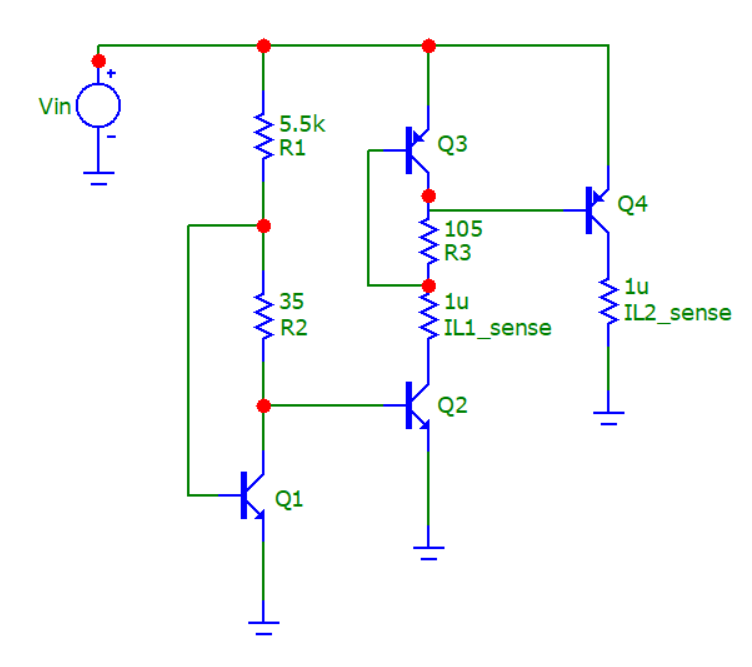
\includegraphics[width=\linewidth]{figures/c3.png} % Image filename
    \centering
    \caption{Circuit Diagram} % Caption
    \label{fig:circuit_Diagram} % Label
\end{figure}

\begin{figure*}[ht]
    \centering
    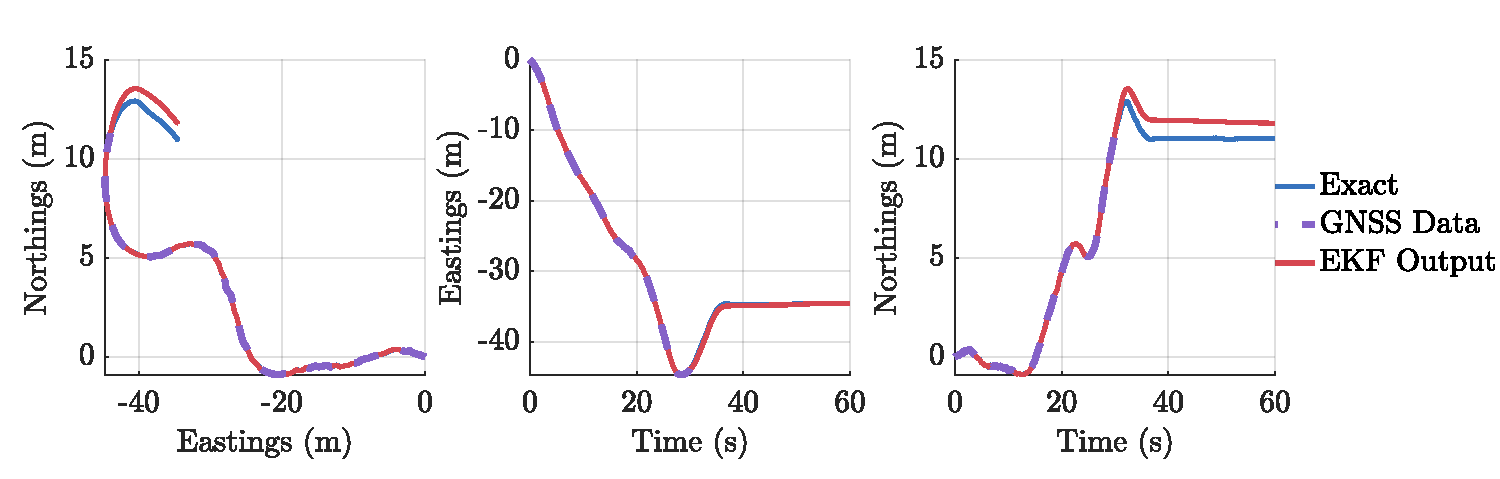
\includegraphics[width=\linewidth]{figures/R6.pdf} % Image filename
    \centering
    \caption{Sick Graphs} % Caption
    \label{fig:sick_graphs} % Label
\end{figure*}


\lstinputlisting[language=Python, caption=Python code, label=code:python_code]{../code/python.py}

\begin{table}[ht]
    \centering
    \begin{tabular}{ccccc}
        \toprule
        \textbf{recording} & 
        \textbf{mean $\Delta \vec{p}$} & 
        \textbf{final $\Delta \vec{p}$} & 
        \textbf{max $\Delta \vec{p}$} \\
        \midrule
        \csvreader[head to column names, late after line=\\]{../data/data.csv}{}
        {\csvcoli & \csvcolii & \csvcoliii & \csvcoliv}
        \bottomrule
    \end{tabular}
    \caption{Summary statistics read from \code{../data/data.csv}}
    \label{table_from_file}
\end{table}



